\documentclass[a4paper,11pt]{article}
\usepackage[utf8]{inputenc}
\usepackage[T1]{fontenc}
\usepackage{geometry}
\usepackage{enumitem}
\usepackage{titlesec}
\usepackage[table]{xcolor}
\usepackage{fancyhdr}
\usepackage{tikz}
\usepackage{tabularx}
\usepackage{listings}
\usepackage{graphicx}
\usepackage{lastpage}
\usepackage{hyperref}

% Page Setup
\geometry{top=1in, bottom=1in, left=0.8in, right=0.8in}
\pagestyle{fancy}
\fancyhf{}
\lhead{\small Project 83: Agentic AI Compiler Assistant}
\rhead{\small Week 9 Report}
\cfoot{\thepage\ of \pageref{LastPage}}

% Formatting
\titleformat{\section}{\Large\bfseries\color{blue!70!black}}{\thesection.}{1em}{}[\titlerule]
\titleformat{\subsection}{\large\bfseries\color{blue!50!black}}{\thesubsection}{1em}{}

% Code Listings
\lstset{
    basicstyle=\ttfamily\small,
    breaklines=true,
    frame=single,
    backgroundcolor=\color{gray!10},
    keywordstyle=\color{blue},
    stringstyle=\color{green!50!black},
    commentstyle=\color{gray},
    showstringspaces=false,
    tabsize=4,
    captionpos=b
}

% Custom commands
\newcommand{\statusgood}[1]{\colorbox{green!20}{\textbf{#1}}}
\newcommand{\statuspending}[1]{\colorbox{yellow!20}{\textbf{#1}}}

\begin{document}

\begin{center}
    {\huge \textbf{Week 9 Progress Report}} \\
    \vspace{3mm}
    {\large \textbf{Project 83: Conversational Agentic AI Compiler Assistant}} \\
    \vspace{2mm}
    \textit{Agentic Tool-Use --- Gemini Function Calling API} \\
    \vspace{2mm}
    \textbf{Reporting Period:} Week 9 | \textbf{Status:} \statusgood{COMPLETED}
\end{center}

\vspace{5mm}

\section{Executive Summary}

Week 9 built the \textbf{Agentic Tool-Use} layer: a set of discrete compiler tools that the Gemini AI agent can autonomously ``call'' using the \textbf{Gemini Function Calling API}, enabling it to investigate code errors step-by-step before producing a final answer.

\textbf{Key Achievement:} The agent now implements the \textbf{ReAct} (Reason $\rightarrow$ Act $\rightarrow$ Observe) loop. Instead of simply receiving a serialized compiler state and responding, Gemini can now dynamically request specific information --- look up a variable's scope, get the full error list, or re-run the pipeline on a proposed fix --- making its debugging process transparent and verifiable.

\subsection{Week Overview}
\begin{itemize}[leftmargin=*]
    \item \textbf{Planned Objectives:} Compiler tool interfaces, Gemini Function Calling integration, ReAct agentic loop, deterministic testing
    \item \textbf{Achieved:} All objectives completed
    \item \textbf{Test Coverage:} 50 new deterministic tests; \textbf{187 total tests passing} (Weeks 5--9)
\end{itemize}

\section{Architecture: Agentic Tool-Use Layer}

\subsection{2.1 Motivation}

In Week 8, Gemini received a static \textit{snapshot} of compiler state at query time. This worked well for known errors but had limitations:
\begin{itemize}
    \item Gemini could not ask follow-up questions about variable definitions
    \item Gemini could not verify whether its suggested fix actually compiles
    \item The debugging process was opaque --- one prompt in, one answer out
\end{itemize}

Week 9 solves this with \textbf{function calling}: Gemini can \textit{request} specific compiler information as part of its reasoning process, and the Python backend executes the appropriate tool and returns the result.

\subsection{2.2 Updated Pipeline}

\begin{table}[h]
\centering
\begin{tabularx}{\textwidth}{|c|l|X|}
\hline
\rowcolor{blue!10}
\textbf{Phase} & \textbf{Component} & \textbf{Output} \\
\hline
Week 5 & Lexer & Token stream \\
\hline
Week 6 & Parser & Abstract Syntax Tree (AST) \\
\hline
Week 7 & Semantic Analyzer & Validated AST + Symbol Table + Errors \\
\hline
Week 8 & Context Provider & Natural Language Context for Gemini \\
\hline
\textbf{Week 9} & \textbf{Compiler Toolbox} & \textbf{7 callable compiler tools} \\
\hline
\textbf{Week 9} & \textbf{Tool Registry} & \textbf{Gemini Function Declarations (schemas)} \\
\hline
\textbf{Week 9} & \textbf{AgenticGeminiClient} & \textbf{ReAct loop with tool-use} \\
\hline
\end{tabularx}
\caption{Compiler pipeline --- Week 9 additions highlighted}
\end{table}

\section{Implementation}

\subsection{3.1 Module: \texttt{src/orchestrator/compiler\_tools.py}}

The \texttt{CompilerToolbox} class exposes seven discrete tools:

\begin{table}[h]
\centering
\begin{tabularx}{\textwidth}{|l|X|}
\hline
\rowcolor{blue!10}
\textbf{Tool} & \textbf{Description} \\
\hline
\texttt{check\_scope(variable\_name)} & Look up a variable in the symbol table; returns type, scope level, and definition line \\
\hline
\texttt{check\_function(function\_name)} & Verify if a function is defined and return its parameter list \\
\hline
\texttt{get\_errors()} & Return all semantic errors with line/column numbers \\
\hline
\texttt{get\_warnings()} & Return all semantic warnings \\
\hline
\texttt{get\_symbol\_table()} & Return the full symbol table (via ContextProvider) \\
\hline
\texttt{get\_ast\_summary()} & Return natural language AST summary (via ContextProvider) \\
\hline
\texttt{reparse\_code(source\_code)} & Re-run the full Lex$\rightarrow$Parse$\rightarrow$Analyze pipeline on new code and update internal state \\
\hline
\end{tabularx}
\caption{CompilerToolbox --- available tools exposed to Gemini}
\end{table}

\begin{lstlisting}[language=Python, caption=CompilerToolbox example: check\_scope()]
def check_scope(self, variable_name: str) -> str:
    symbol = self.analyzer.symbol_table.lookup(variable_name)
    if symbol is None:
        return f"SCOPE CHECK: '{variable_name}' is NOT defined in any scope."
    return (
        f"SCOPE CHECK: '{variable_name}' is defined.\n"
        f"  Type: {symbol.symbol_type.value}\n"
        f"  Defined at: line {symbol.line}, column {symbol.column}"
    )
\end{lstlisting}

All tools return plain-text strings. Gemini receives these as ``observations'' in the ReAct loop. The \texttt{dispatch(tool\_name, args)} method routes tool calls by name.

\subsection{3.2 Module: \texttt{src/orchestrator/tool\_registry.py}}

The Tool Registry translates the toolbox into \textbf{Gemini Function Declaration schemas} --- JSON-style objects that tell Gemini what tools exist, what parameters they take, and what they do:

\begin{lstlisting}[language=Python, caption=Tool registry schema example (check\_scope)]
{
    "name": "check_scope",
    "description": "Look up a variable in the compiler's symbol table...",
    "parameters": {
        "type": "object",
        "properties": {
            "variable_name": {
                "type": "string",
                "description": "The variable name to look up"
            }
        },
        "required": ["variable_name"]
    }
}
\end{lstlisting}

The \texttt{build\_gemini\_tools()} function converts these dicts into \texttt{genai.protos.Tool} objects for the Gemini API. A plain-dict fallback is used for testing without API access.

\subsection{3.3 Class: \texttt{AgenticGeminiClient}}

The \texttt{AgenticGeminiClient} extends \texttt{GeminiCompilerAgent} (Week 8) and adds:

\begin{enumerate}
    \item \textbf{\texttt{investigate\_with\_tools()}}: Main entry point. Builds the initial investigation prompt and starts the ReAct loop.
    \item \textbf{\texttt{\_agentic\_loop()}}: Drives the ReAct cycle with a \texttt{MAX\_ITERATIONS = 8} safety cap.
    \item \textbf{\texttt{simulate\_agentic\_investigation()}}: Fully offline simulation of the agentic behavior --- no API key required. Used for testing and demos.
\end{enumerate}

\section{The ReAct Loop}

The \textbf{ReAct} (Reason + Act) pattern works as follows:

\begin{center}
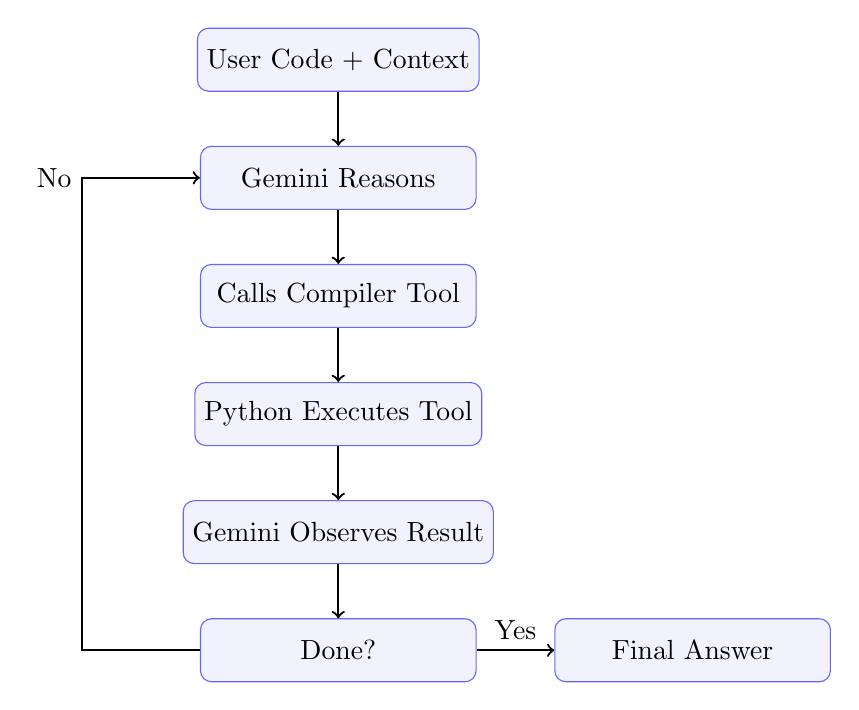
\begin{tikzpicture}[
    node distance=1.5cm,
    box/.style={rectangle, draw=blue!60, fill=blue!5, rounded corners, minimum width=3.5cm, minimum height=0.8cm, text centered},
    arrow/.style={->, thick}
]
\node[box] (start) {User Code + Context};
\node[box, below of=start] (reason1) {Gemini Reasons};
\node[box, below of=reason1] (toolcall) {Calls Compiler Tool};
\node[box, below of=toolcall] (execute) {Python Executes Tool};
\node[box, below of=execute] (observe) {Gemini Observes Result};
\node[box, below of=observe] (decide) {Done?};
\node[box, right of=decide, xshift=3cm] (answer) {Final Answer};

\draw[arrow] (start) -- (reason1);
\draw[arrow] (reason1) -- (toolcall);
\draw[arrow] (toolcall) -- (execute);
\draw[arrow] (execute) -- (observe);
\draw[arrow] (observe) -- (decide);
\draw[arrow] (decide) -- node[above]{Yes} (answer);
\draw[arrow] (decide.west) -- ++(-1.5,0) |- node[left]{No} (reason1.west);
\end{tikzpicture}
\end{center}

\textbf{Example session} for code: \texttt{total = price * quantity + discount}

\begin{enumerate}
    \item Gemini calls \texttt{get\_errors()} $\rightarrow$ sees 3 undefined variable errors
    \item Gemini calls \texttt{check\_scope("price")} $\rightarrow$ ``NOT defined''
    \item Gemini calls \texttt{check\_scope("quantity")} $\rightarrow$ ``NOT defined''
    \item Gemini calls \texttt{reparse\_code(fixed\_code)} $\rightarrow$ ``SUCCESS''
    \item Gemini produces final answer with explanation and fixed code
\end{enumerate}

\section{Testing \& Validation}

\subsection{5.1 Test Suite Summary}

\begin{table}[h]
\centering
\begin{tabularx}{\textwidth}{|l|c|X|}
\hline
\rowcolor{blue!10}
\textbf{Test Class} & \textbf{Tests} & \textbf{Focus Area} \\
\hline
TestCompilerToolboxCheckScope & 7 & Defined/undefined vars, type, scope level, line number \\
\hline
TestCompilerToolboxCheckFunction & 5 & Functions with/without params, undefined, variable $\neq$ function \\
\hline
TestCompilerToolboxGetErrors & 5 & No errors, single/multiple errors, line numbers, count \\
\hline
TestCompilerToolboxGetWarnings & 2 & No warnings, type-change warning \\
\hline
TestCompilerToolboxGetSymbolTable & 4 & Global scope, variables, functions, multiple vars \\
\hline
TestCompilerToolboxGetAstSummary & 3 & Structure header, function, assignment \\
\hline
TestCompilerToolboxReparse & 5 & Valid/invalid code, state update, replace old state \\
\hline
TestToolDispatch & 8 & All 7 tools + unknown tool error \\
\hline
TestToolRegistry & 8 & Schema completeness, names, descriptions, parameters \\
\hline
TestAgenticSimulation & 7 & Return dict, tool calls made, valid/error answers, observations \\
\hline
TestToolboxIntegration & 5 & Full pipeline valid/error, reparse fix, factory, function check \\
\hline
\textbf{Total (Week 9)} & \textbf{59} & \textbf{All passing, fully deterministic (no API calls)} \\
\hline
\textbf{Grand Total} & \textbf{187} & \textbf{Weeks 5--9, all passing} \\
\hline
\end{tabularx}
\caption{Week 9 Test Suite}
\end{table}

\subsection{5.2 Key Design Decision: Deterministic Tests}

All 59 new tests run without any Gemini API calls. The \texttt{AgenticGeminiClient.simulate\_agentic\_investigation()} method mimics the ReAct loop deterministically, allowing full coverage of the agentic pipeline in CI/CD without API access.

\section{Deliverables}

\begin{itemize}[leftmargin=*]
    \item \statusgood{COMPLETE} \texttt{src/orchestrator/compiler\_tools.py} --- CompilerToolbox with 7 tools + dispatch
    \item \statusgood{COMPLETE} \texttt{src/orchestrator/tool\_registry.py} --- Function declaration schemas for all tools
    \item \statusgood{COMPLETE} \texttt{src/orchestrator/gemini\_client.py} --- AgenticGeminiClient with ReAct loop
    \item \statusgood{COMPLETE} \texttt{tests/test\_week9\_tools.py} --- 59 deterministic tests
    \item \statusgood{COMPLETE} \texttt{demo\_week9\_agentic.py} --- 6-section demo (5 offline + 1 optional API)
    \item \statusgood{COMPLETE} \texttt{reports/week\_09\_report.tex} --- This report
\end{itemize}

\section{Challenges \& Solutions}

\subsection{7.1 Deterministic Testing of Agentic Behavior}
\textbf{Problem:} The ReAct loop depends on Gemini deciding which tools to call, making it non-deterministic.

\textbf{Solution:} Implemented \texttt{simulate\_agentic\_investigation()} which deterministically runs the same tool sequence (get\_errors $\rightarrow$ get\_symbol\_table $\rightarrow$ get\_ast\_summary $\rightarrow$ check\_scope for each error) without API calls. This allows testing all tool logic and observation formatting while keeping the live API loop available for production use.

\subsection{7.2 Backward Compatibility}
\textbf{Problem:} Extending \texttt{GeminiCompilerAgent} risked breaking Week 8 behavior.

\textbf{Solution:} Used subclassing --- \texttt{AgenticGeminiClient extends GeminiCompilerAgent}. All Week 8 methods (\texttt{analyze\_with\_context}, \texttt{explain\_error}, \texttt{get\_assistance}) remain unchanged and all 128 prior tests still pass.

\subsection{7.3 API Library Deprecation}
\textbf{Problem:} The \texttt{google-generativeai} package is deprecated in favor of \texttt{google-genai}.

\textbf{Solution:} The existing codebase already uses \texttt{google-generativeai} throughout; migration to the new SDK is tracked as a future task. Current functionality is unaffected.

\section{Next Week Preview}

\textbf{Week 10: Conversational Debugging Interface}

\begin{itemize}[leftmargin=*]
    \item Build a multi-turn chatbot CLI/UI for step-by-step error explanation
    \item Maintain conversation history across multiple user queries
    \item Implement follow-up question handling
\end{itemize}

\section{Conclusion}

Week 9 successfully implemented the \textbf{Agentic Tool-Use} layer, enabling the Gemini AI agent to autonomously investigate code errors using seven discrete compiler tools via the Function Calling API. The ReAct loop allows Gemini to reason, act (call a tool), observe the result, and reason again --- transforming it from a passive analyzer into an active debugging agent. All 187 tests pass with the existing 128 tests fully preserved.

\vspace{5mm}
\noindent\textbf{Prepared by:} Project Team \\
\textbf{Reporting Date:} Week 9 Completion (10 March 2026) \\
\textbf{Next Review:} Week 10 Report

\end{document}
